\subsection{Der globale Anwendungszustand}

\begin{figure}[H]
    \centering
    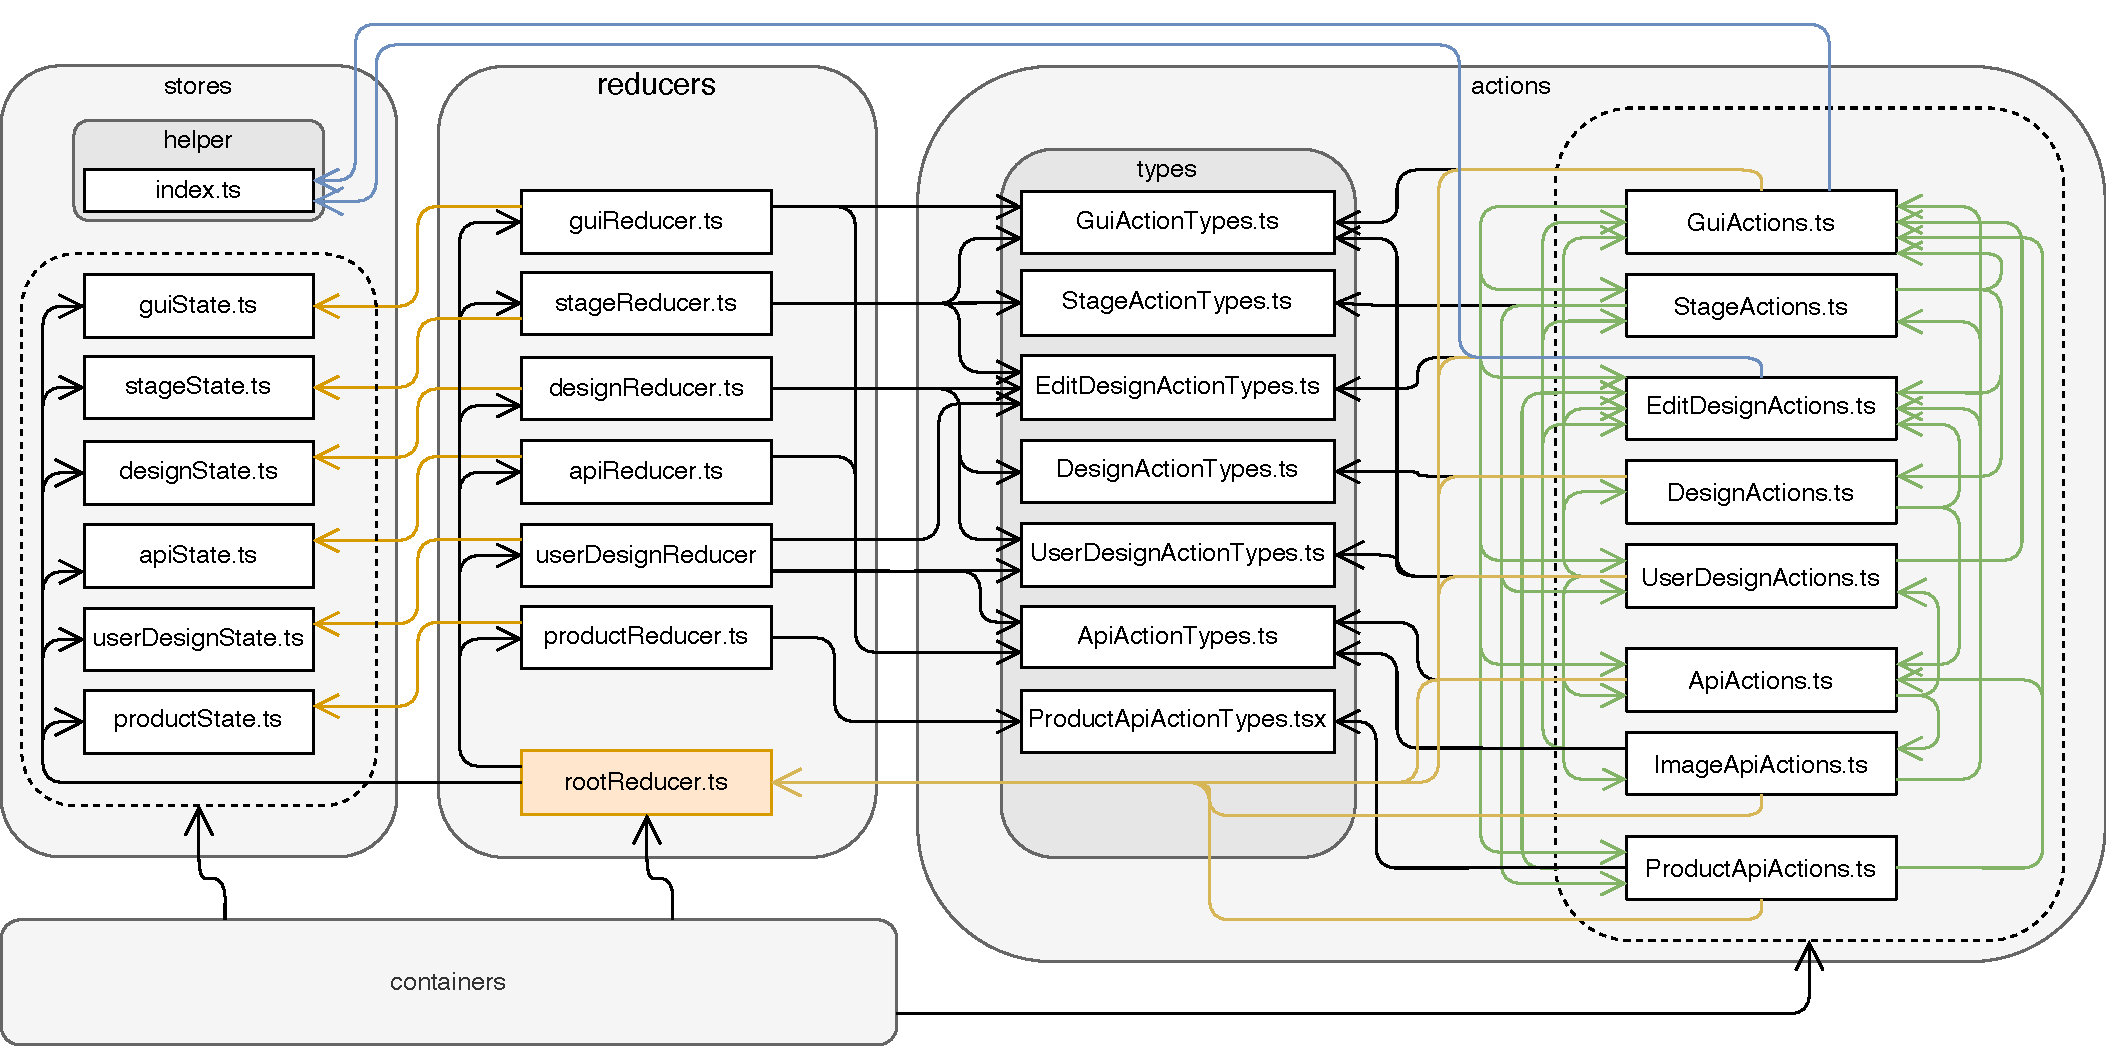
\includegraphics[width=1\textwidth]{diagrams/Ist-Architektur/Redux.pdf}
    \caption{Darstellung der Zusammenhänge zwischen den \lstinline|store| \lstinline|actions| und \lstinline|reducers|}
    \label{fig:Redux}
\end{figure}




\begin{filecontents}{\jobname-storetable.tex}
\newcommand{\minitab}[2][l]{\begin{tabular}{#1}#2\end{tabular}}
    
\begin{longtable}{l|X}
\textbf{Schnittstelle} & \textbf{Beschreibung} \\ 
\hline 

\multirow{2}*{\minitab{IGuiState  \\ \lstinline|stores/guiState.ts|}}    & 
Beschreibung des Zustands der grafischen Oberfläche des FreeDesign-Editors. 
Beispiele hierfür sind die Darstellung von modalen Dialogen oder der Aufbau der Menüs. 

\\

\multirow{2}*{\minitab{IStageState     \\  \lstinline|stores/stageState.ts| }}      & 
Vom Zustand der grafischen Oberfläche entkoppelt, wird durch die Schnittstellen \lstinline|IStageState| der Zustand der zentralen Oberfläche zur Produktbearbeitung (Stage) beschrieben.

\\ 

\multirow{2}*{\minitab{IProductState  \\   \lstinline|stores/productState.ts| }}   & 
Die Zustandsbeschreibung des Produkts welches der Nutzer bearbeiten enthält, sowohl Information für Darstellung innherhalb des FreeDesign-Editors, als Informationen die für den Bestellprozess relevant sind.

\\

\multirow{2}*{\minitab{IDesignState   \\   \lstinline|stores/designState.ts| }}     & 
Beschreibung des Designs welches der Nutzer bearbeiten. Desweiteren wird durch den Zustand eine Historie der Bearbeitungsschritte gepflegt.

\\

\multirow{2}*{\minitab{IApiState  \\ \lstinline|stores/apiState| }}           & 
    Die bereits genannten Zustände, \lstinline|IProductState|, \lstinline|IDesignState|, \lstinline|IUserDesignState| und \lstinline|IUserState| werden von Werte belegt, die durch API bereitgestellt werden. Allerdings besitz der \emph{Redux-State} ein weiteres Unterobjekt, welches durch die Schnittstelle  \lstinline|IApiState| beschrieben wird und ebenfalls durch Daten der API beschrieben wird. Hierzu zählt eine Liste von Schriftarten, die innerhalb eines Designs genutzt werden können, sowie eine Liste der Bilder, die ein Kunde in seinem Design nutzt.  

\\

\multirow{2}*{\minitab{ICoreState   \\  \lstinline|@unitedprint/frontend-core|}} & 
    Der Zustand \lstinline|core| wird vom Quelletext nicht genutzt und wurde mutmaßlich vergessen bei einem Refactoring zu entfernen.

\\

\multirow{2}*{\minitab{IUserState   \\  \lstinline|@unitedprint/frontend-core| }} & 
    Die Struktur enthält Informationen des Nutzers, wie Kundenart oder Rechnungs- und Lieferaddresse. 

\\

\multirow{2}*{\minitab{ ITranslationsState \\ \lstinline|@unitedprint/frontend-core| }} & 
    \lstinline|ITranslationsState| enthält eine Liste der Texte für die grafische Oberfläche.
\\

\multirow{2}*{\minitab{IUserDesignState \\ \lstinline|stores/userDesignState|  }}   & 
Für das Verwalten von Metadaten eines Kundendesigns, wie der Designname unter dem ein Design gespeichert wurde oder der Zeitstempel, wann ein Design erstellt, wird durch die Schnittstelle \lstinline|IUserDesignState| beschrieben.
\\

\end{longtable}
\end{filecontents}
\LTXtable{\textwidth}{\jobname-storetable.tex}